\chapter{Rare earth element distributions and trends in natural waters with a focus on groundwater}
\chaptermark{REE in natural waters}

This chapter is adapted from a publication by the same name, co-authored by David A. Dzombak and Athanasios K. Karamalidis.
This paper is citable as: 

Noack, C. W.; Dzombak, D. A.; Karamalidis, A. K., Rare Earth Element Distributions and Trends in Natural Waters with a Focus on Groundwater. \textit{Environ. Sci. Technol.} \textbf{2014}, \textit{48}, (8), 4317-4326.

\clearpage

\section*{Abstract}
Systematically varying properties and reactivities have led to focused research of the environmental forensics capabilities of the rare earth elements (REE).
Increasing anthropogenic inputs to natural systems may permanently alter the natural signatures of REEs, motivating characterization of natural REE variability.
We compiled and analyzed reported dissolved REE concentration data over a wide range of natural water types (groundwater, ocean-, river-, and lake water) and groundwater chemistries (e.g. fresh, brine, and acidic) with the goal of quantifying the extent of natural REE variability, especially for groundwater systems.
Quantitative challenges presented by censored data were addressed with non-parametric distributions and regressions.
Reported measurements of rare earth elements in natural waters range over nearly ten orders of magnitude, though the majority of measurements are within two to four orders of magnitude, and are highly correlated with one another.
Few global correlations exist among dissolved abundance and bulk solution properties in groundwaters indicating the complex nature of source-sink terms and the need for care when comparing results between studies.
This collection, homogenization, and analysis of a disparate literature facilitates inter-study comparison and provides insight into the wide range of variables that influence REE geochemistry.


\section{Introduction}

In the natural sciences, predictable thermodynamic differences between the rare earth elements (REE) allow for interpretation of natural geologic and chemical processes \citep{REE_dep_study, REE_soil_tracers}. 
Rare earth lithogeochemistries have long been used to infer depositional environments of geologic strata \citep{REE_dep_study, PAAS, Hanson_EPS_1980}.
Similarly, REE serve as benign analogs to the transuranic actinides for nuclear waste disposal studies \citep{Krauskopf_CG_1986, Millero_GCA_1992} and for studying mixing and metal cycling in the oceans \citep{DeBaar_Nat_1983, Elderfield_PTRS_1988}.
These characteristics make REE attractive tools for environmental forensic applications such as pollutant source identification and apportionment \citep{Kulkarni_AE_2006, Kulkarni_EST_2007}.

Based on atomic number, the REE are segregated into light and heavy REE (LREE and HREE, respectively) with the division occurring between Eu and Gd \citep{Castor_Hedrick};
some studies also distinguish middle REE (MREE), though the specific elements are inconsistently defined between authors \citep{Hannigan_CG_2001, Tang_CG_2010, Choi_CG_2009, Brookins_RMG_1989}.
These ``weight'' distinctions allow for simplified description and quantification of the inter-element relationships, typically ratios of normalized concentrations, which are exploited in REE analysis.
Similarly, anomalies of certain REE -- due to redox lability for Ce and Eu \citep{Brookins_RMG_1989} and large anthropogenic emissions for Gd \citep{Bau_EPSL_1996} -- are used to interpret geochemical processes. 
Y and Sc exhibit similar properties to the lanthanides and are thus included in the suite of REE with Y being most similar to HREE and Sc being most similar to LREE in solution \citep{Brookins_RMG_1989}.
 
Aquatic geochemists apply the same principles used by geologists, the inter-element ratios and anomalies described previously, to infer water-rock interactions, hydrologic connectivity between geologic units, and groundwater mixing members \citep{Johannesson_GCA_1997, Johannesson_GW_1997, BwireOjiambo_AG_2003, Siebert_AG_2012}.
Interactions with different mineral phases have been shown to alter REE patterns predictably.
For example, an MREE enrichment is observed for fresh waters in contact with phosphate-rich minerals \citep{Hannigan_CG_2001} while HREE enrichment is found in carbonate-rich waters \citep{Johannesson_EPSL_1996}.
Tester et al. \citep{Tesmer_HJ_2007} showed that groundwater end-members, especially at shallow depths, could be established by interpretation of REE patterns.
Similarly, REE concentrations have been used to calculate end-member contributions to groundwater \citep{Johannesson_GCA_1997, BwireOjiambo_AG_2003}.
 
The capabilities of REE to serve as tracers of groundwater migration and mixing have potential applications to the study of hydrology and geochemistry of shale gas development or the capture and sequestration of carbon dioxide (CO$_2$) gas in geologic formations.
For example, characteristic REE profiles could possibly enable detection of brines displaced from shale or CO$_2$ storage zones and into overlying groundwater aquifers \citep{Benson_Cole, Karamalidis_EST_2012, Chaudhuri_JOCGS_2011, Cheung_IJCG_2009}.
Capable tools for contaminant detection, as well as contaminant source apportionment, are critical to the long-term environmental feasibility of these technologies.
Increasing anthropogenic inputs of REE to the environment threaten to obfuscate natural signals, which would complicate these applications \citep{Kulaksiz_EI_2011, Kulaksiz_EPSL_2013}.

A primary challenge in analyzing REE data, like other geochemical compositional data \citep{Palarea_CompData_2011}, is the prevalence of censored observations, defined as values below the analytical method detection limit (MDL) or a value excluded due to excessive analytical interferences.
Appropriate statistical methodologies, largely borrowed from survival analysis (or reliability analysis), allow for analysis of these data without relying on substitution or interpolation \citep{Helsel_EST_1995}.
Utilizing these techniques removes the bias of left-censored data and of uneven sample sizes from summary statistics and statistical inference \citep{Helsel_EST_1995, Helsel_EST_2005}. 

Significant contributions to the understanding of REE geochemistry in natural waters have been made through critical review of thermodynamics \citep{Brookins_RMG_1989, Wood_CG_1990},
catchment-scale case studies \citep{Dia_GCA_2000, Gruau_WR_2004, Pourret_AG_2010, Ma_CG_2011},
and groundwater flow system studies \citep{Johannesson_GCA_1997, Johannesson_GCA_1999, Johannesson_CG_2000, Tang_CG_2006, Willis_CG_2011} among others.
Lacking thus far in the REE literature is the aggregation and analysis of the numerous and disparate studies of the REE and the origin of their concentrations.
Such a compilation would enhance inter-study comparison through internal consistency, allow for investigation of broader trends, and enhance statistical analysis by increasing sample sizes.

In this work, a compilation and analysis of data from independent studies of REE in natural waters was performed, focusing on trends in groundwaters.
The study focused on shallow groundwaters well as some deeper groundwaters capable of impacting surface water or shallow groundwater.
The compiled data were used to develop a consistent database of REE concentrations and their associated major solute chemistry and to explore interelement relationships, examine trends in REE abundance, and test hypotheses related to REE abundance as functions of major solution chemistry parameters.
The objectives of this work were: (1) to ascertain an expected range of dissolved REE concentrations in waters of variable chemistries, deriving unbiased estimates of REE distributions and (2) to investigate trends in REE abundance in groundwater in relation to other available chemical parameters (e.g. pH, ionic strength, and major solution species).

\section{Methods}

\subsection{Data assimilation and criteria}

The low-temperature, aqueous REE systematics were investigated by extracting available REE concentration data in reported studies of ground-, sea-, river-, and lake waters.
Data were gathered from these studies for dissolved REE concentrations (defined here as constituents passing through a 0.45 \si{\um} filter). 
Many studies filter at finer pore sizes in order to study colloidal association \citep{Dia_GCA_2000, Pourret_JCIS_2007, Stolpe_GCA_2013},
however 0.45 \si{\um} was chosen because it is a common size for groundwater analysis and  maximized the number of samples available.
While REE are commonly defined to include Y and Sc, very few studies measured Y and almost none examined Sc.
Therefore, our analyses of REE focused on the 14 naturally abundant lanthanides (excluding the short-lived, radioactive Pm).
In total, 31 studies with 619 samples were collected for groundwater,14, 19, 20, 22, 33-35, 37-40, 43-63
16 studies with 178 samples for seawater,7, 45, 64-77
16 studies with 259 samples for river water,12, 19, 48, 67, 71, 78-89
and 8 studies with 74 samples for lake water.19, 56, 57, 82, 85, 90-92

A significant literature exists for other water types, for example mine drainage \citep{Borrego_HR_2012, Bozau_AG_2004, Doulati_JEE_2013, Romero_AG_2010, Verplank_AG_2004, Worrall_GCA_2001, Zhao_IJCG_2007} and hydrothermal waters/hot springs \citep{Haas_GCA_1995, Lepel_conf_1988, Michard_GCA_1989, Lewis_GCA_1997, Lewis_GCA_1998, Sanada_Geotherm_2006}.
However, these water types have been excluded from this study in order to focus on waters minimally impacted by anthropogenic activity (in the case of mine drainage) and that occur broadly with chemistry dominated by near-surface pressure, temperature, and mineralogical conditions (in the case of hydrothermal waters/hot springs).

\subsection{Analysis of censored data}

In the accumulated dataset, 18\% of all REE measurements were either below detection or missing.
For individual elements in different waters, up to 52\% of measurements were censored (Tm in groundwater).
The censoring rates of each element, in each water type, are given in Figure~\ref{fig:cen_frac}.
Given this high frequency, it was necessary to employ modified statistical methods to handle this type of information31 and avoid creating a false data signal either by substitution (i.e., one-half MDL) or interpolation.

\begin{figure}[htbp]
\begin{center}
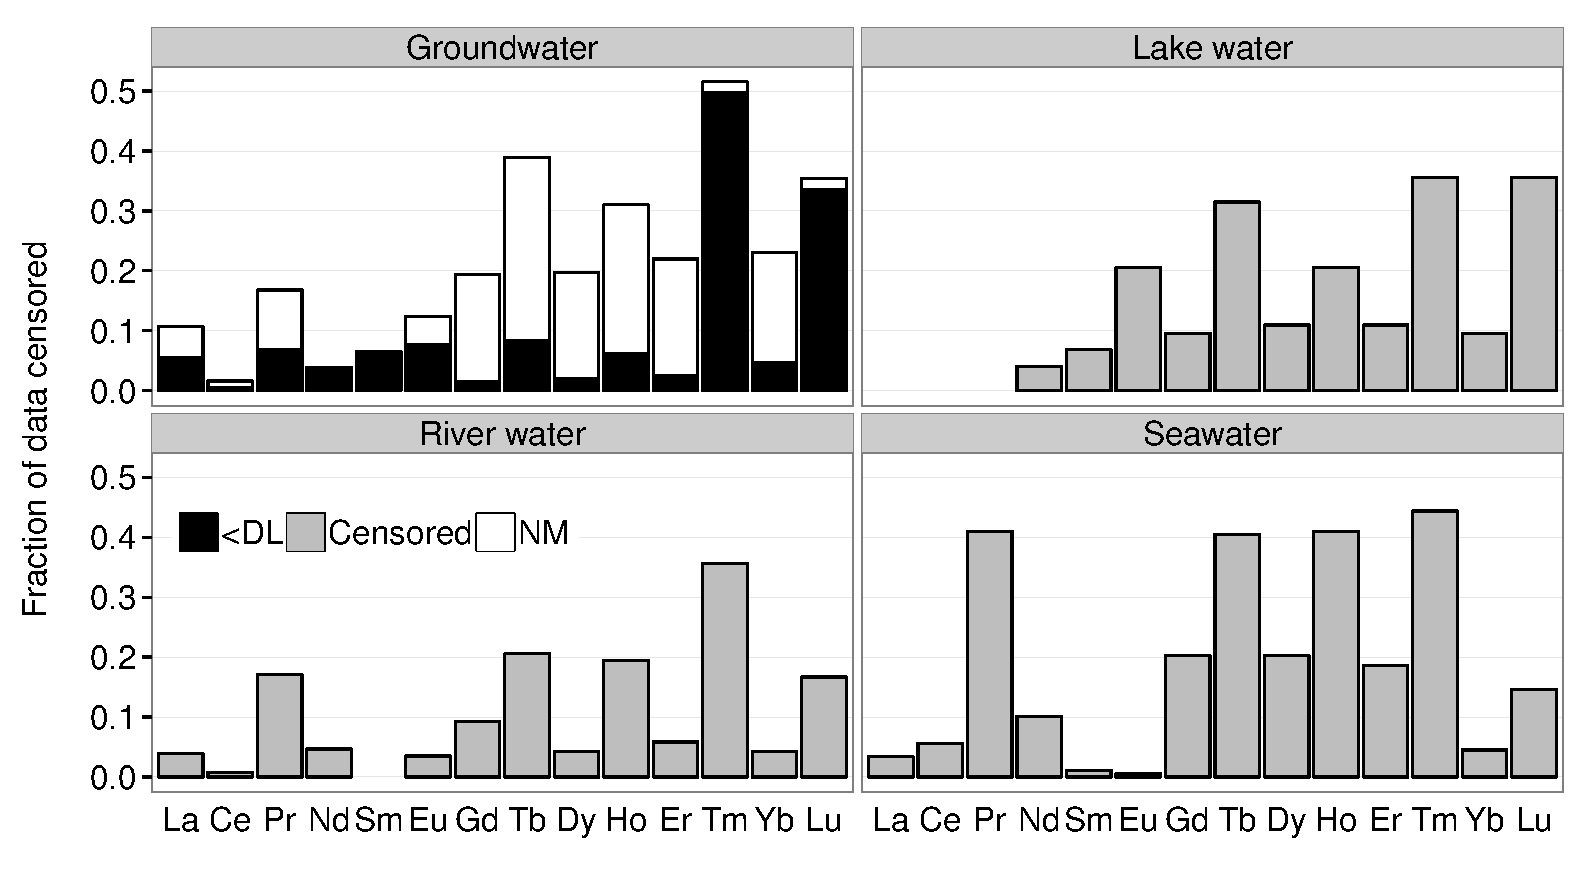
\includegraphics[width=\textwidth]{Ch3_figures/REE-waters-nonDet-type.pdf}
\caption{Fraction of below detection limit ($<$DL) or missing data (NM) for 14 REE in data sets for water types studied. For water types other than groundwater, censored data were not differentiated as below detection or missing, and are lumped together as ``censored''.}\label{fig:cen_frac}
\end{center}
\end{figure}


An additional complexity of this data set was the uneven distribution of data points between data sets (Figure~\ref{fig:sample_dist}).
For example, some data sets included more than seventy samples, while other contained fewer than ten.
This uneven distribution can bias calculated statistics towards studies with a higher number of samples, giving larger studies more weight than smaller studies \citep{Singh_JAWMA_2013}.

\begin{figure}[htbp]
\begin{center}
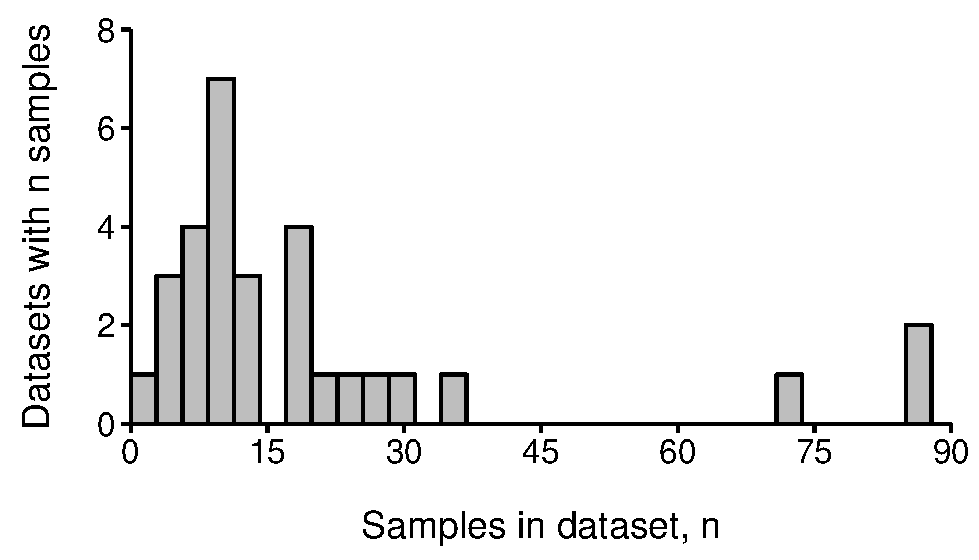
\includegraphics[width=0.8\textwidth]{Ch3_figures/cite-n-dist.pdf}
\caption{Histogram of sample distribution in groundwater dataset (compiled from 31 articles).}\label{fig:sample_dist}
\end{center}
\end{figure}

Censored data were stored at the study-specific MDL with a separate binary variable indicating that the data were censored. Missing data -- that is where REE were either not measured, not reported, or where an MDL was not specified -- were excluded from calculations because nothing was known about the data point in relation to the rest of the data.

Summary statistics were calculated using a weighted Kaplan-Meier (KM) estimator of the survival function accounting for both left-censored and source-size bias.
A routine based on the methodology of Singh, et al. \citep{Singh_JAWMA_2013} was written in \texttt{R} \citep{R} to perform the necessary calculations.
Distribution percentiles were estimated as the first value with a calculated percentile less than the percentile of interest;
stated differently, if the calculated survival quantiles, $S(x)$, for adjacent observations were $S(x_1)=0.94$ and $S(x_2)=0.96$, then $x_1$ would be noted as the 95$^{th}$ percentile.
For data sets with a limited number of samples (e.g. brines) where the sample size or censoring frequency limited the number of calculable percentiles, a log-normal distribution was fit to the KM survival curve by regression on order statistics (ROS) and was used to estimate those percentiles.
Mean values, $\mu_{KM}$, were calculated from the area under the survival curve and standard deviations, $\sigma_{KM}$, from the variance of the mean \citep{Helsel_book}.

The survival curve was approximated using a weighted KM estimator, which considers non-detect data and provides robustness to the uneven distribution of samples from the reviewed literature.
Equation~\ref{eq:wKM} represents the weighted KM estimator, where $\hat{S}(x_i)$ is the probability any observation from the dataset will be \textit{less than} the measured concentration, $x_i$.
In this equation $d_i^w$ represents the weighted count of uncensored observations at concentration $x_i$ and $Y_i^w$ represents the weighted count of all (censored and uncensored) observed concentrations less than $x_i$.
The weight, $w_i$, of each observation is the inverse of the number of samples from the data source ($n_i$), or: $w_i = n_i^{-1}$.
In the absence of weighting or censoring, this formula reduces to the empirical cumulative distribution function.
These calculations, and the relevant \texttt{R} code, are discussed algorithmically in Appendix \textbf{A}.

\begin{align}\label{eq:wKM}
\hat{S}(x_i) = \prod_{x_i>x}\left(1 - \frac{d_i^w}{Y_i^W} \right)
\end{align}

Uncertainty in this estimate, expressed using Greenwood's formula \citep{Helsel_book}, is defined by Equation~\ref{eq:greenwood}. As with Equation~\ref{eq:wKM}, $d_i^w$ represents the weighted count of uncensored observations at concentration $x_i$ and $Y_i^w$ represents the weighted count of all observed concentrations less than $x_i$.

\begin{align}\label{eq:greenwood}
\sigma_{\hat{S}}(x_i) = \hat{S}(x_i)\sqrt{\Sigma_{j=1}^k\frac{d_j^w}{Y_j^w (Y_j^w - d_j^w)}}
\end{align}

Total dissolved REE concentrations were calculated with consideration of censored data.
Rather than calculating the KM survival curve and $\mu_{KM}$ for an individual element (where each sample is an observation) the survival curve was calculated for individual samples (where each REE is an observation).
The sum was determined as follows \citep{Helsel_book}:

\begin{align}\label{eq:totalREE}
\Sigma [REE] = 14\times \mu_{KM}
\end{align}

 
In addition to univariate summary statistics, inter-element correlations are significantly influenced by the high degree of censoring within the REE data.
Using Pearson's r (linear, least-squares correlation) as an estimate of the correlation would require substitution for censored or missing values \citep{Helsel_EST_1995}.
Instead, the Spearman's $\rho$ statistic enabled incorporation of censored data, diminished the influence of outliers (by being robust to log-transformation), and assessed monotonic relationships beyond simple linear relationships.

\bibliographystyle{unsrtnat}
\bibliography{Ch3_bib_edit}




